% !TeX encoding = UTF-8
% !TeX root = MAIN.tex

\chapter{Motivation}


The starting point of this thesis is recently conducted research which studies the link and causal effects between monetary policy decisions by the FED and stock market in the U.S.  not only in an ex-post,  but moreover in an ex-ante sense.

The paper "Stock Returns over the FOMC Cycle" \parencite{cieslak_stock_2019} finds that "the equity premium is entirely earned in even weeks starting from the last FOMC meeting (0,  2,  4 and 6)" which implies that the FED has "overly affected the stock market via unexpectatly accommodating policy". 

Another paper "The Economics of the FED Put"  \parencite{cieslak_economics_2020} uses textual analysis of FOMC scripts to identify and measure the causal effect that policy makers indeed pay intention to the "stock market" and negative stock returns are linked with downgrades in growth projections (in an ex-post sense) since the mid-1990s.  
Although policy makers seem to be aware of that the so-called "FED put" "could induce risk-taking" the paper concludes that it does not "significantly affect their decision-making in an ex-ante sense".


\chapter{What is the "Fed Put" and how can it be explained?}


The "Fed put" refers to the Federal Reserve's perceived policy of intervening in the financial markets to prevent a sharp decline in asset prices.  \parencite{rosenblum_fed_2007}
This term is derived from the concept of a "put option",  which is a financial instrument that gives the holder the right, but not the obligation,  to sell an asset at a predetermined price..
The Fed put suggests that the Federal Reserve will step in to prevent a market decline,  much like a put option would protect an investor from the decline in the value of an asset. 

The Federal Reserve's intervention in the financial markets has been a topic of debate among economists and market investors. 
The term "Greenspan Put" is often used to describe the perceived tendency of the Federal Reserve,  under the leadership of former Chairman Alan Greenspan,  to intervene in financial markets in order to prevent significant declines or disruptions. 
Some argue that market interventions are necessary to prevent financial crises,  while others believe that these interventions distort the market and create moral hazards.  \parencite{cieslak_economics_2020}

The FED's role as the lender of last resort function of the Federal Reserve has initially been established to provide liquidity to the financial system during times of stress.  \parencite{holland_role_1991}
This means that the Federal Reserve stands ready to lend money to financial institutions to prevent systemic collapse. 

However, the "Fed put" goes beyond the lender of last resort function,  as it suggests that it will also intervene in the markets to prevent a steep decline in asset prices.
Therefore some believe that the Fed put has created a moral hazard in the markets.  \parencite{rosenblum_fed_2007} 
This means that investors are willing to take on excessive risks because they believe that the Federal Reserve will always bail them out.  
Critics argue that this creates a "too big to fail" mentality among investors and can lead to financial crises in the long run. 

During the 2008 financial crisis,  the Federal Reserve implemented several programs to provide liquidity to the financial system and prevent a collapse of the financial system. 
These programs,  such as the Term Auction Facility and the Term Asset-Backed Securities Loan Facility,  were designed to stabilize the markets.  

Similarly,  in March 2020, when the COVID-19 pandemic caused a sharp decline in the financial markets,  the Federal Reserve quickly implemented several measures to support the markets,  including cutting interest rates to near-zero and implementing a program of unlimited quantitative easing \parencite{powell_monetary_2021}.


\textbf{Chapter summary}

In conclusion,  the Fed put remains a controversial and important concept when it comes to modern monetary policy.  
The Federal Reserve's intervention in the financial markets has been a topic of debate among economists and investors,  as some argue that these interventions are necessary to prevent financial crises,  while others believe that they create moral hazards. 

\chapter{Does the stylized fact of stock excess returns are mainly achieved in FOMC even weeks (0,  2,  4,  6) from 2016 onwards still persist?}

Empirical part I

\chapter{Is there empirical evidence for a similar effect when considering only the euro-zone and euro-zone stock returns.  Does it imply an equivalent of the Fed Put in the Euro-Zone?}

Empirical part II

\begin{figure}[h]
    \centering
    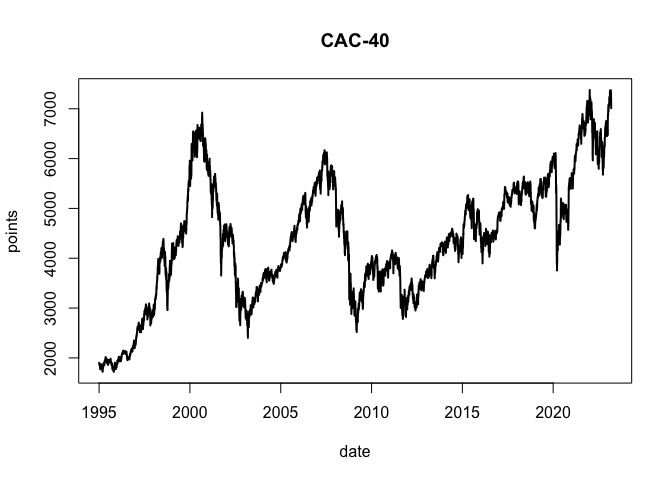
\includegraphics[width=0.9\textwidth]{figures/cac-40}
    \caption{CAC-40 Index from 3rd january 1995 to 27th march 2023}
\end{figure}

\chapter{Conclusion}


